\documentclass[a4paper,11pt]{scrartcl}
\usepackage[utf8x]{inputenc}
\usepackage[catalan]{babel}
\usepackage{titlesec}
% A ses llengües llatines, el primer paràgraf ha d'anar tabulat
\usepackage{indentfirst}
\usepackage{amsmath}
\usepackage{float}
\usepackage{graphicx}
\usepackage{subfigure}
\usepackage{booktabs}
\usepackage{multirow}
\usepackage{hyperref}
\usepackage{url}
\usepackage{multirow}
\usepackage{minted} %wget http://minted.googlecode.com/hg/minted.sty

% aptitude install texlive-fonts-extra
\usepackage{newcent} %font mes wapa

\graphicspath{{diagrames/}}

% Estil de seccions
\titleformat{\section}{\large\sectfont}{\thesection}{1em}{}
\titleformat{\subsection}{\bfseries\sectfont}{\thesubsection}{1em}{}
% Estil numeracio subseccions http://help-csli.stanford.edu/tex/latex-sections.shtml#number
%\def\thesubsection{\alph{subsection})}

\title{Robòtica: \\ Rainer\footnote{Explicació de que vol dir rainer} \ Project}
\author{ Bartomeu Miró Mateu \thanks{bartomeumiro a gmail punt com} \\
	 Lluis Cortès Rullan \thanks{lluisbinet a gmail punt com} }

\begin{document}

  \maketitle

  \begin{abstract}
    Segona pràctica de Robòtica de l'apartat de robòtica mòbil.
    Programació d'una arquitectura de control per un robot Pioneer-3DX que
    permeti moure’s per un entorn amb obstacles i realitzar una determinada
    tasca.
  \end{abstract}

  \newpage
  \setcounter{page}{2}
  \tableofcontents
  \newpage

  \section{Interpretació de l'enunciat}

En l'enunciat es descriu essencialment com dur a terme l'evitació d'obstacles i finalment
es proposen una sèrie de tasques a implementar com ara recorrer un conjunt de punts, vagar etc.

En aquesta pràctica s'implementa un robot netejador que vendria a ser un eufemisme per dir un
robot que intenta cobrir tots els punts d'una determinada àrea evitant els obstacles.

A banda d'aquesta funció principal també s'ha implementat la funcionalitat de vagar.

En aquesta implementació no es destaca l'originalitat de l'acció duita a terme (robot de neteja)
sinó que s'ha intentat fer èmfasi em la jerarquia de l'arquitectura i l'encapsulat de les funcions de tal
manera que un cop establert això és molt senzill desenvolupar noves tasques o afegir i modificar
funcionalitats, tema que es torna a tractar en l'apartat de possibles ampliacions.
  \section{Càlculs}
En aquest apartat explicam com ho fa el robot per calcular la direcció que a de
seguir i com ho fa per evitar els obstacles. Existeixen diferents tècniques,
però com indica l'enunciat em utilitzat comportaments reactius, més concretament
els camps de potencial. 

Un comportament és un mòdul que a partir d'una sèrie d'estimuls dóna una
resposta determinada. Com em comentat aquests comportaments són reactius, per
tant no es realitza cap tipus de planificació i només depen de les dades que es
tenen en cada instant. 

Existeixen diferents formes d'implementar els comportaments. A n'aquesta
pràctica em utilitzat els camps de potencial. Els camps de potencial són un
mètode que consisteix en modelitzar el robot com si fos una partícula sotmesa a
forces. Cada comportament generara una força i la direcció del robot s'obtindrà
a partir de la suma ponderada del resultat de cada comportament.

Els comportaments que s'han implementat són el d'anar cap a un objectiu i el
d'evitar obstacles. El primer produeix un vector d'atracció cap al punt
objectiu. El segon, per cada sensor que detecta un objecte produeix un vector
de repulsió. Llavors, aquets dos vectors es combinen i s'obté el vector
resultant que ens indicarà la direcció a la qual s'ha de dirigir el robot. 

\subsection{Càlcul vector d'atracció}

\subsection{Càlcul vector de repulsió}

\subsection{Càlcul vectro director} 





  \section{Estructura del programa}

  \section{Joc de proves}

Per tal de provar la pràctica s'han realitzat una sèrie de jocs de proves
descrits a continuació. Per cada un d'ells s'ha generat un mapa amb el
\emph{Mapper3Basic} i es poden trobar a la carpeta \emph{maps}.

Al \texttt{Makefile} es troben totes les opcions comentades a l'apartat \emph{sim}, així doncs
es descomenta la desitjada i es comenta la que està per defecte. A continuació
es canvia el codi font
de \texttt{rainer.cpp} comentant el cleanArea i descomentant l'opció desitjada.
Un cop fet això amb un \emph{make} és compila el codi i amb el \emph{make sim}
s'executa el simulador.

El primer test és simple, \textbf{passar per quatre punts sense cap obstacle}. Amb aquest simplement es comprova que es calculi
bé el vector d'atracció. També es pot observar si el \emph{heading} es fa de
manera adequada. Per fer aquesta execució no s'empre cap mapa.

\begin{figure}[H]
\begin{center}\label{4punts}
 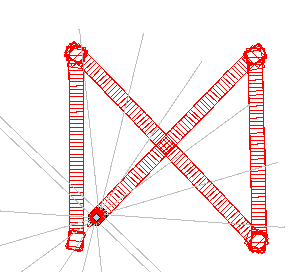
\includegraphics[width=0.5\textwidth]{diagrames/figures/4punts.png}
 % ordreRotacions.png: 1286x768 pixel, 150dpi, 21.77x13.00 cm, bb=0 0 617 369
\end{center}
  \caption{Quatre puts sense obstacle}
\end{figure}

En segon lloc tenim \textbf{passar per quatre punts però amb un obstacle}
enmig. En aquest es veu si l'esquiva d'obstacles es fa bé. A més l'obstacle està
co\lgem ocat de tal manera que el robot es troba impactant una línia de 45 graus
amb el punt destí a la perpendicular, de tal manera que seria una situació
delicada on quedar-se estancat. Per fer aquesta execució s'empra el mapa
\emph{obstacleInclinat}.

\begin{figure}[H]
\begin{center}\label{4puntsObs}
 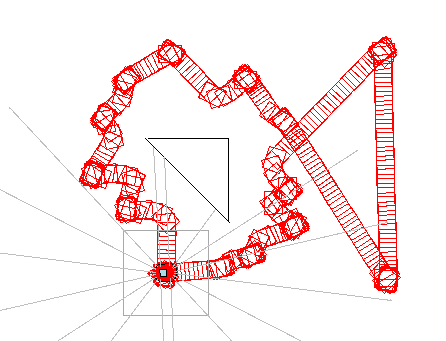
\includegraphics[width=0.5\textwidth]{diagrames/figures/4puntsObs.png}
 % ordreRotacions.png: 1286x768 pixel, 150dpi, 21.77x13.00 cm, bb=0 0 617 369
\end{center}
  \caption{Quatre puts sense obstacle}
\end{figure}

A continuació trobam el mateix \textbf{obstacle} però aquest cop \textbf{situat sobre el punt de destí}, en aquest cas
el robot ha de detectar que no pot arribar-hi ja que l'obstacle i el punt de
destí estan per davall d'un cert llindar. Fins que no s'assoleix aquest llindar
es veu com el robot intenta fer aproximacions al punt desde diferents
direccions. En aquest test empram el mapa \emph{obstacleApunt}.

\begin{figure}[H]
\begin{center}\label{obsapunt}
 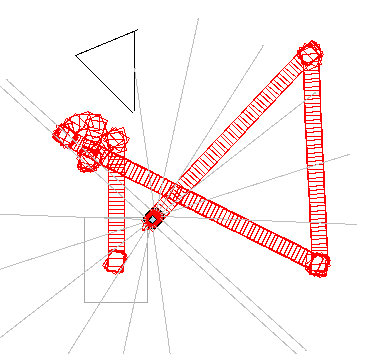
\includegraphics[width=0.5\textwidth]{diagrames/figures/obsapunt.png}
 % ordreRotacions.png: 1286x768 pixel, 150dpi, 21.77x13.00 cm, bb=0 0 617 369
\end{center}
  \caption{Quatre puts sense obstacle}
\end{figure}

Per tal de provar el \textbf{vagar} tenim un mapa tancat amb diversos obstacles
on el robot va rebotant.
Pot arribar un punt en que el robot entri en un cicle ja que els angles de rebot
poden fer que així coincideixi. El que no es permet es que el robot toqui un
obstacle o es quedi immòbil sols girant sobre ell mateix sense ser capaç de
emprendre la ruta cap a una altra banda.

\begin{figure}[H]
\begin{center}\label{vagant}
 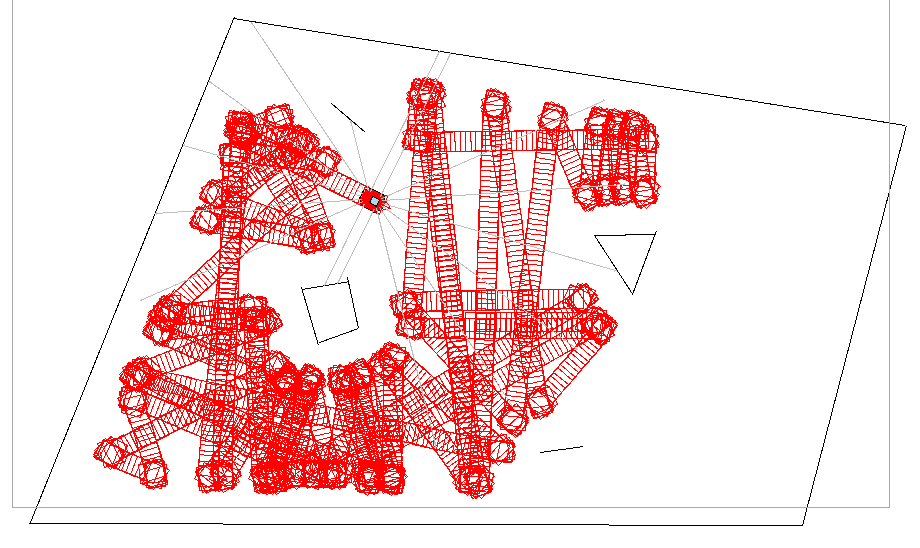
\includegraphics[width=0.5\textwidth]{diagrames/figures/vagant.png}
 % ordreRotacions.png: 1286x768 pixel, 150dpi, 21.77x13.00 cm, bb=0 0 617 369
\end{center}
  \caption{Quatre puts sense obstacle}
\end{figure}

A continuació tenim les proves de la \textbf{neteja de zona}, la primera \textbf{sense obstacles} per veure el recorregut.

\begin{figure}[H]
\begin{center}\label{neteja}
 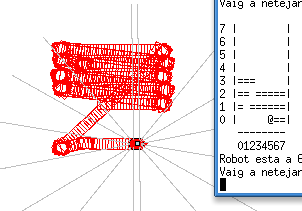
\includegraphics[width=0.5\textwidth]{diagrames/figures/netNoObs.png}
 % ordreRotacions.png: 1286x768 pixel, 150dpi, 21.77x13.00 cm, bb=0 0 617 369
\end{center}
  \caption{Quatre puts sense obstacle}
\end{figure}

I finalment la \textbf{neteja amb obstacles} on el robot els esquiva (i marca terreny durant aquesta esquiva)
i com finalment torna a les zones d'obstacle per comprovar que no fos un
obstacle mòbil i ara si que pot netejar la zona. En aquest últim no podem
simular obstacles mòbils però si veure com torna a intentar anar a la zona
obstaculitzada.

\begin{figure}[H]
\begin{center}\label{netejaobs}
 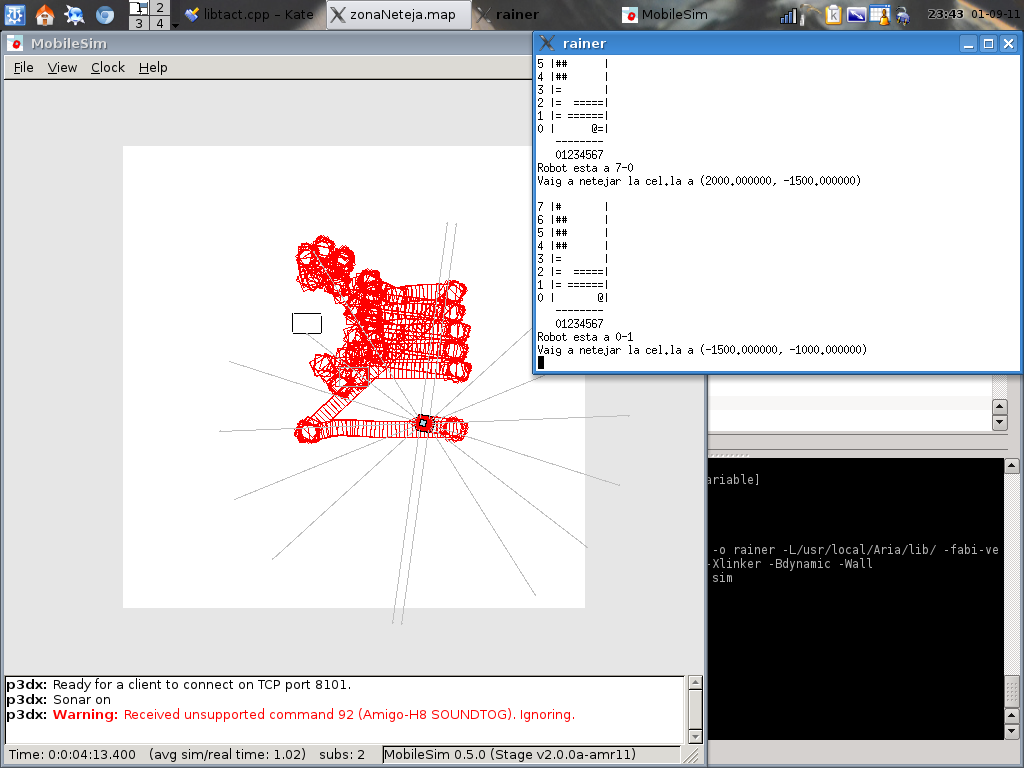
\includegraphics[width=0.5\textwidth]{diagrames/figures/netejant.png}
 % ordreRotacions.png: 1286x768 pixel, 150dpi, 21.77x13.00 cm, bb=0 0 617 369
\end{center}
  \caption{Primera passada de la neteja}
\end{figure}

\begin{figure}[H]
\begin{center}\label{figescenari}
 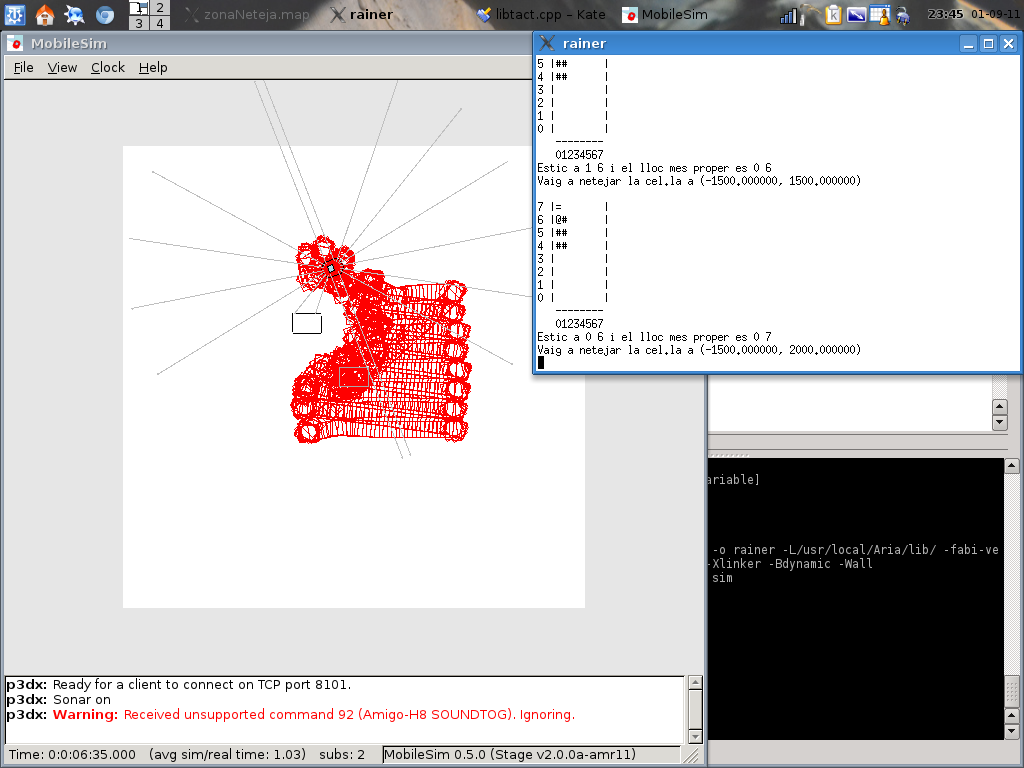
\includegraphics[width=0.5\textwidth]{diagrames/figures/netejant-aobstacles.png}
 % ordreRotacions.png: 1286x768 pixel, 150dpi, 21.77x13.00 cm, bb=0 0 617 369
\end{center}
  \caption{Segona passada de la neteja anant als punts detectats com obstacle}
\end{figure}


  \section{Incidents, problemàtica al desenvolupament i valoració}\label{incidents}

Durant el desenvolupament com es habitual hom es troba amb problemes a resoldre,
alguns d'ells fruit de l'aprenentatge però d'altres deguts a limitacions
de l'entorn ja sigui físic com virtual.

\subsection{Problemàtica física}


\subsection{Problemàtica virtual}

\subsection{Valoració}

 \let\thefootnote\relax\footnotetext{
 Aquest document està baix llicència \href{http://creativecommons.org/licenses/by-sa/3.0/}{Creative Commons Atributive Share-Alike 3.0}
 per tant es pot compartir, modificar i distribuir, però citant els autors originals i sense modificar la llicència.
 De la mateixa manera el codi font està baix llicència GNU GPL v3 per part dels dos autors.\bigskip}
\let\thefootnote\relax\footnotetext{El document en versió digital i el codi font el trobareu a \\
\url{https://github.com/bmiro/rainer}\bigskip}
\let\thefootnote\relax\footnotetext{Aquest document i tota la part de la practica que s'ha pogut ha estat desenvolupat emprant programari lliure:}
\let\thefootnote\relax\footnotetext{\href{http://www.tug.org/applications/pdftex/}{\LaTeX} i \href{http://www.tug.org/applications/pdftex/}{Kile} per el text,
\href{http://www.inkscape.org/}{Inkscape} pels diagrames,
\href{http://kate-editor.org/}{Kate} i \href{http://vim.org/}{Vim} per l'edició del codi font.
\href{http://git-scm.com/}{Git} com a sistema de control de versions.
}

\let\thefootnote\relax\footnotetext{
\begin{center}
\begin{tabular}{cc}

\includegraphics[height=35pt,keepaspectratio=true]{diagrames/by-sa.png}
 & 
\includegraphics[height=35pt,keepaspectratio=true]{diagrames/gnu.png}
\end{tabular}
\end{center}
\begin{center}
\begin{tabular}{cccccc}
 
\includegraphics[height=35pt,keepaspectratio=true]{diagrames/latex.png}
 & 
\includegraphics[height=35pt,keepaspectratio=true]{diagrames/kile.png}
 & 
\includegraphics[height=35pt,keepaspectratio=true]{diagrames/inkscape.png}
 & 
\includegraphics[height=35pt,keepaspectratio=true]{diagrames/kde.png}
 & 
\includegraphics[height=35pt,keepaspectratio=true]{diagrames/vim.jpg}
 & 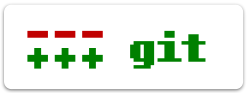
\includegraphics[height=35pt,keepaspectratio=true]{diagrames/git.png}
\end{tabular}
\end{center}
}

  \section{Annex: Codi font complet}

\subsection{Rainer, cos principal}
\inputminted[linenos, frame=lines, fontsize=\footnotesize]{cpp}{../rainer.cpp}
\newpage
\subsection{librainer, llibreria de l'estratègic}
\inputminted[linenos, frame=lines, fontsize=\footnotesize]{cpp}{../librainer.h}
\inputminted[linenos, frame=lines, fontsize=\footnotesize]{cpp}{../librainer.cpp}
\newpage
\subsection{libtact, llibreria del nivell tàctic}
\inputminted[linenos, frame=lines, fontsize=\footnotesize]{cpp}{../libtact.h}
\inputminted[linenos, frame=lines, fontsize=\footnotesize]{cpp}{../libtact.cpp}
\newpage
\subsection{librainermap, llibreria transversal del mapa}
\inputminted[linenos, frame=lines, fontsize=\footnotesize]{cpp}{../librainermap.h}
\inputminted[linenos, frame=lines, fontsize=\footnotesize]{cpp}{../librainermap.cpp}
\newpage
\subsection{lib2d, llibreria transversal d'aritmètica de vectors i punts}
\inputminted[linenos, frame=lines, fontsize=\footnotesize]{cpp}{../lib2d.h}
\inputminted[linenos, frame=lines, fontsize=\footnotesize]{cpp}{../lib2d.cpp}

\end{document}
